\subsection{General iterative work}
The simulations are performed with C++. The code is available in an online git repository \newline https://www.github.com/zfg663/simulating-omnivory.

The initial food web consists of a basic nutrient source and a primary producer feeding on the source, and evolves through additions of invasive species. After each invasion the food web is allowed to settle before a new invasion takes place. Each simulation conducts $10^5$ invasions.
\begin{algorithm}
\SetAlgoLined
%\KwResult{Write here the result }
 initializing food web\;
 \While{invasions < $10^5$}{
  add species\;
  compute steady states\;
  \If{steady states > 0}{
   compute linear stability\;
   }  
   
  \While{not settled}{
    integrate food web\;
  }
  }
 \caption{Overall procedure}
 \label{CODE:procedure}
\end{algorithm}
With each invasion $\bf{S^*}$ is computed, and if the food web is found to be feasible also the linear stability is computed with matrix operations from the Eigen library \cite{eigen} (Algorithm \ref{CODE:procedure}). 
% Necessary to explain why?
% "The stability and feasibility are used to determine state of food web". Not really clear..
The integration is performed with 4th order Runge-Kutta \cite{atkinson2008introduction} and adaptive step size of the Runge-Kutta-Fehlberg method \cite{}.

% necessary to explain different scenarios?
% if unfeasible, then
% if feasible, then stab of unstab....
For each time step the food web is checked for extinct species. A species, $S$ is considered extinct if $S \leq 10^{-12}$ % approximately $10^2-10^4$ times the precision of the type 'double' in C++ \cite{dowd2010high}.
After an extinction $\bf{S^*}$ and linear stability are computed again (Algorithm \ref{CODE:extinction}). %and time is set to zero.
\begin{algorithm}
\SetAlgoLined
\While{state unknown}{
 integrate food web\;
 ... \newline
 \If{density $\leq\:10^{-12}$}{
  remove species\;
  compute steady states\;
  compute linear stability\;
 }
 ...
}
 \caption{Check for extinction}
 \label{CODE:extinction}
\end{algorithm}

If the food web is feasible and linearly stable the densities are compared to $\bf{S^*}$, breaking the integration if the densities are found to converge in $\bf{S^*}$.

\begin{algorithm}
% how detailed about softening criterion?
% not done!
\SetAlgoLined
\While{state unknown}{
 integrate food web\;
 ... \newline
 \If{feasible \textbf{and} linearly stable}{
 \If{|density / $\bf{S^*}$ - $\bf{S^*}$| $\leq\:10^{-6}$}{
    break\;
 }
 }
 ...
}
 \caption{Check for convergence}
 \label{CODE:convergence}
\end{algorithm}
The criterion is softened if the food web takes longer than $t = ^5\cdot10^4$ %verify
to converge.

If the food web is not linearly stable, a test for periodic oscillations is carried out.
%% NOT DONE

Hence, invasive species are only added to feasible food webs. In that sense the procedure imitates the natural selection of evolution, as the species that is better fit will outperform and kill the weaker species. However, in this simulation fitness is measures relative to the structure of the food web. An illustration of the procedure can be seen in Figure \ref{FIG:evolution}.

\begin{figure}
    % pick oscillatory/"chaotic" food webs
    % add 0.5 to density plots (linear, not logarithmic...)
    \centering
		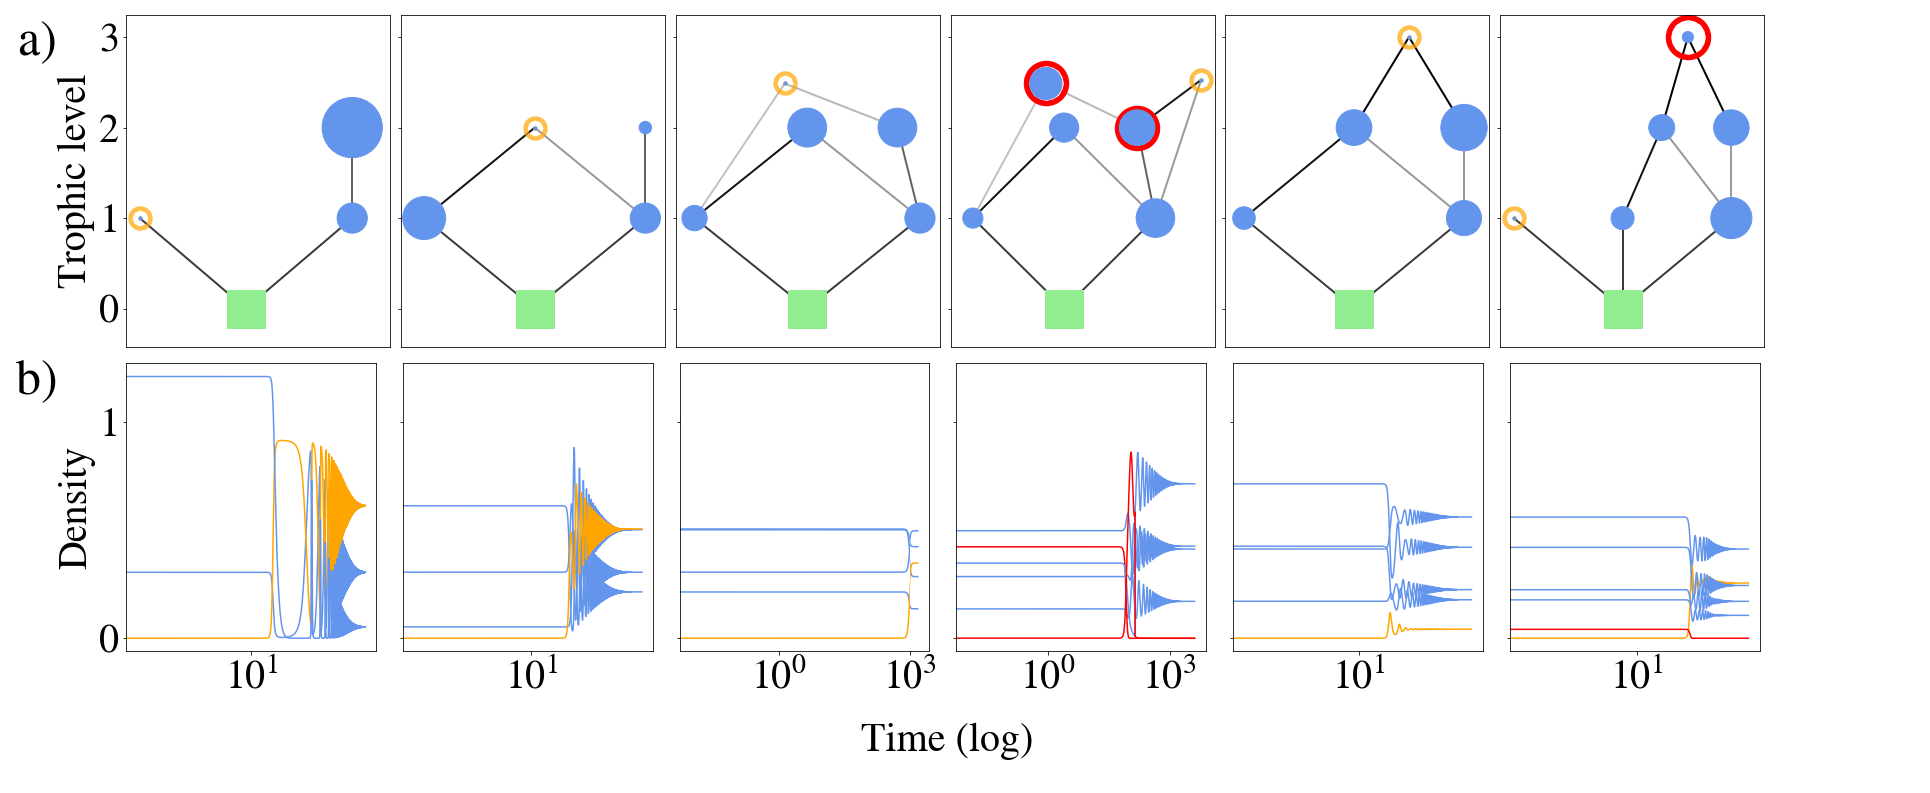
\includegraphics[scale = 0.13]{figs/evolution.png}
	    \caption{\textbf{Time series of a food web during 6 invasions.} \textbf{a)} 6 addition attempts on a food web corresponding to addition 260, 263-266, 268. The orange and red circles denote the invasive and extinct species, respectively. 
        The area corresponds to the density of the species, and the color of the edge corresponds to the interaction strength between two species, where a dark edge corresponds to strong interaction. The green square is the basic nutrient source. \textbf{b)} The corresponding time series of the food webs above on a logarithmic time scale. 
        The line colors correspond to the species' colors in a), i.e. the red and orange curves represent the species that become extinct and invades the food web. The blue lines represent the other species. All 6 food webs are stable. To be changed...}
	    \label{FIG:evolution}
\end{figure}

\subsection{Declaring a species}
\begin{figure}
% what is difference between class diagram and object        diagram
% not done!
    \centering
    \includegraphics[width = 0.5\textwidth]{figs/class_diagram.pdf}
    \caption{A class diagram of species and producer. To be improved!!}
    \label{FIG:class}
\end{figure}
Species are represented by objects in the code.
A class 'species' is created, with the derived class 'producer' containing the subgroup of primary producers. 
In the following species and producer will denote a member of the class of the same name unless otherwise stated. Each member of species (hence also of producer) contains a density variable, species- and link-specific parameters and a trophic level, corresponding to $S_i, k_i, \alpha_i, \eta_{ji}, \beta_{km}$ and $l_i$ from eq. (\ref{eq:LV_i}) and (\ref{eq:LV_k}).
Furthermore, each member contains a function for computing its time-derivative, $\dot{S_i}$, that is eq. (\ref{eq:LV_i}) or (\ref{eq:LV_k}) multiplied by $S_i$ for producers and species, respectively. When a species is declared, it is assigned a small initial density, $S = 10^{-10}$, and species-specific parameters from different distributions. For simplicity $k_i = 1$ for all producers. $\alpha \in \mathcal{U}(0.05, 0.5)$, as high decay rates are believed to be outperformed by lower. Something about $\beta$.
The resulting parameters $\eta_{ji}$ and $l$ depend on the dynamics of the specific food web, and will be assigned to the species as it is added to the food web. The declaration ratio of producers to species is 1:2. % might change this


\subsection{Addition of a species}
\begin{table}[width=.9\linewidth, cols=2, pos=h]
    \caption{Table containing all parameters and their distributions. NB: might change these}
    \label{TBL:parameters}
    \begin{tabular*}{\tblwidth}{L@{} LLL@{} }
        \toprule
        Parameter & Distribution \\
        \midrule
        $k$ & 1 \\
        $\alpha$ & $\mathcal{U}(0.05, 0.5)$ \\
        $\eta$ & $\mathcal{U}(0.05, 1)$ \\
        ... & ...\\
        \bottomrule
    \end{tabular*}
\end{table}
A species is added to the food web with the creation of interactions with the food web. For a producer this interaction is the consumption of the basic nutrient source, whereas the species is assigned at least one resources among the resident species.
A second link is established with probability $1/2$ for species invading food webs of $3$ or more species. When a link is created $\eta_{ki}$ is drawn from $\eta \in \mathcal{U}(0.05, 1)$.
The invader is allowed to consume any species and is not limited by its trophic level, as this is computed only after it is linked to the food web. The trophic level is computed from
\begin{equation}
    l_k = 1 + \frac{1}{n_{r}}\frac{\sum_m^{n_{r}} \eta_{km}l_m}{\sum_m^{n_{r}} \eta_{km}}.
    \label{eq:l}
\end{equation}
Here $l_m$ is the level of a resource species and $n_{r}$ is the total number of resources of a species. 
The trophic levels of all species are updated before each invasion, as a resource species of a species might have gone extinct since last invasion. Accordingly, they are also updated after each invasion, because existing species might be consuming the invasive species. 

The resource species of the invasive species are drawn from a uniform distribution. 
Although it is argued that a species chooses resources after availability or specializes on a certain type of resource species \cite{sih1990interacting}, this is not imitated in the simulation.
This also reflects the fact that this model does not allow a species to mutate or in other ways adapt to changes in its environment. 
The steady states of a species might change drastically as the web evolves. 
Hence, should a species pick resources after to quantity, it should also be able to adapt to changes in the resource population.
